% !TEX program = xelatex
% 中心科学实验 IV 研究型实验报告

\documentclass[a4paper]{article}

% ===== 字体 =====
\usepackage{fontspec}
\usepackage{xeCJK}
\setCJKmainfont[BoldFont=SimHei]{SimSun}
\setCJKsansfont[BoldFont=SimHei]{SimHei}
\setCJKmonofont{FangSong}
\newCJKfontfamily\heiti[BoldFont=SimHei]{SimHei}
\newCJKfontfamily\kaishu{STKaiTi}
\newCJKfontfamily\fangsong{STFangSong}
\newCJKfontfamily\xingkai{STXingkai}
\xeCJKsetup{AutoFakeBold=true}
\setmainfont{Latin Modern Roman}

% ===== 字号定义 =====
\newcommand{\zihaoSan}{\fontsize{16pt}{24pt}\selectfont}
\newcommand{\zihaoSi}{\fontsize{14pt}{21pt}\selectfont}
\newcommand{\zihaoWu}{\fontsize{10.5pt}{16pt}\selectfont}
\newcommand{\zihaoXiaoWu}{\fontsize{9pt}{13.5pt}\selectfont}
\newcommand{\zihaoLiu}{\fontsize{7.5pt}{11pt}\selectfont}

\usepackage{setspace}
\usepackage[a4paper,top=4.6cm,bottom=3.0cm,left=2.5cm,right=2.0cm,headheight=3.8cm,headsep=0.8cm,footskip=1.8cm]{geometry}
\usepackage{fancyhdr}
\usepackage{graphicx}
\usepackage{booktabs}
\usepackage{multirow}
\usepackage{caption}
\usepackage[super,sort&compress]{natbib}
\bibliographystyle{unsrt}
\usepackage[colorlinks=true,linkcolor=black,urlcolor=blue,citecolor=black]{hyperref}
\usepackage{indentfirst}
\usepackage{enumitem}
\usepackage{needspace}

\captionsetup[table]{labelsep=space,font={small},position=above,skip=4pt,justification=centering}
\captionsetup[figure]{labelsep=space,font={small},position=below,skip=4pt,justification=centering}
\setlength{\parindent}{2em}
\setlength{\parskip}{0pt}
\setlist{nosep}

% ===== 页眉页脚 =====
\newcommand{\infobar}{%
  \zihaoWu
  \setlength{\tabcolsep}{0pt}%
  \vspace{0.5em}
  \begin{tabular}{@{}p{0.315\textwidth}p{0.315\textwidth}p{0.315\textwidth}@{}}
    系（Dept.）\underline{\hspace{2.2cm}} &
    专业（Major）\underline{\hspace{1.3cm}} &
    学号（ID）\underline{\hspace{1.3cm}} \\[7pt]
    姓名（Name）\underline{\hspace{1.6cm}} &
    日期（Date）\underline{\hspace{1.5cm}} &
    实验台号（No.）\underline{\hspace{0.8cm}}
  \end{tabular}%
  \vspace{1em}
}

\newcommand{\myhead}{%
  \begin{minipage}[c]{2cm}%
    
\includegraphics[height=2cm]{template/images/img-000.png}%
  \end{minipage}%
  \vspace{-0.5em}%
  \begin{minipage}[c]{\dimexpr\textwidth-1.8cm\relax}%
    \centering
    {\hspace{-1.5em}\zihaoSan\heiti 中心科学实验 IV\hspace{2em}{\xingkai 实\kern0.2em 验\kern0.2em 报\kern0.2em 告}}\\[3pt]
    {\hspace{-1.5em}\fontsize{11pt}{14pt}\selectfont\textbf{Experimental Report of Central Science}}\\[6pt]
    \infobar
  \end{minipage}%
}

\pagestyle{fancy}
\fancyhf{}
\renewcommand{\headrulewidth}{0.4pt}
\renewcommand{\footrulewidth}{0.4pt}
\fancyhead[L]{\myhead}
\fancyfoot[C]{\vspace{-0.5em}\zihaoWu \bfseries 化学国家级实验教学示范中心（厦门大学）\\[1pt]{\textbf{\fontsize{9pt}{13pt}\selectfont National Demonstration Center for Experimental Chemistry Education (Xiamen University)}}}
\fancypagestyle{plain}{\fancyhf{}\renewcommand{\headrulewidth}{0.4pt}\renewcommand{\footrulewidth}{0.4pt}\fancyhead[L]{\myhead}\fancyfoot[C]{\vspace{-0.5em}\zihaoWu \bfseries 化学国家级实验教学示范中心（厦门大学）\\[1pt]{\textbf{\fontsize{9pt}{13pt}\selectfont National Demonstration Center for Experimental Chemistry Education (Xiamen University)}}}}

\usepackage{titlesec}
\titleformat{\section}{\zihaoSi\heiti}{\thesection}{1em}{}
\titlespacing{\section}{0pt}{12pt}{6pt}
\titleformat{\subsection}{\zihaoWu\heiti\bfseries}{\thesubsection}{1em}{}
\titlespacing{\subsection}{0pt}{0pt}{0pt}

\begin{document}
\setstretch{1.05}
\zihaoWu

\begin{center}
  {\zihaoSan\heiti 无机贵金属纳米粒子的合成及表征}
\end{center}
\vspace{6pt}

\section{引言}
\vspace{-0.5em}

贵金属纳米粒子因其尺寸、形貌和表面状态可调，表现出明显不同于块体金属的光学与表面化学性质。金、银纳米粒子的典型特征是局域表面等离激元共振（localized surface plasmon resonance, LSPR）：入射光驱动导带电子发生集体振荡，使纳米粒子在可见光区产生强吸收和散射。LSPR 峰位与粒径、形貌、组成、分散状态及周围介质密切相关，因此同为金属金或银，纳米尺度样品可呈红、黄、灰绿等不同颜色，而不再呈现宏观金属的金黄色或银白色\cite{Willets2007,Mayer2011}。

贵金属纳米粒子的制备常采用液相还原法。以柠檬酸钠为代表的温和还原剂既可将金属离子还原为零价金属，又可吸附在颗粒表面提供静电和空间位阻稳定作用。根据 LaMer 成核--生长模型，若反应初期形成足够高的单体过饱和度，可在短时间内集中成核，随后主要发生晶核长大，从而获得粒径相对集中的胶体颗粒。相较一步法，晶种法先制备小尺寸晶种，再在较低过饱和度下控制外延生长，有利于调控粒径和各向异性形貌，但步骤更多、对反应条件更敏感\cite{Pratap2025,CoreShell2025}。

本实验围绕金、银纳米粒子的合成、形貌观察与光谱应用展开。扫描电子显微镜（SEM）用于直接观察粒子形貌、尺寸和团聚状态；拉曼光谱用于鉴别钻石、翡翠等样品；表面增强拉曼光谱（surface-enhanced Raman spectroscopy, SERS）进一步利用贵金属纳米粒子表面的电磁增强和“热点”效应，实现孔雀石绿等分子的痕量检测\cite{Zhou2023,Deniz2019}。通过将 SEM 与拉曼/SERS 结果结合，可以理解纳米粒子的结构特征如何影响其光学响应和分析检测能力。

\section{实验部分}
\vspace{-0.5em}

\subsection{仪器与试剂}

实验使用氯金酸、硝酸银、柠檬酸钠、孔雀石绿、碘化钠及去离子水等试剂制备和表征贵金属纳米粒子。主要仪器包括加热搅拌装置、离心机、扫描电子显微镜、紫外--可见分光光度计和教学型拉曼光谱仪。拉曼测试采用约 531.8 nm 激光激发；常规样品测试积分时间为 1 s，电化学原位 SERS 序列积分时间为 100 ms。

\subsection{实验方法}

\textbf{金、银纳米粒子的一步法制备。} 将金盐或银盐水溶液加热至沸腾，在搅拌条件下加入柠檬酸钠溶液。反应过程中柠檬酸根逐步还原金属离子，并在新生纳米粒子表面吸附以抑制进一步聚并。金纳米粒子体系由浅黄色逐渐转为红色，银纳米粒子体系由无色或浅色逐渐转为灰绿或灰蓝色，颜色变化反映了等离激元吸收带的形成及粒径/聚集状态变化。

\textbf{形貌与光学表征。} 合成后的胶体经离心清洗后滴加于导电基底，干燥后进行 SEM 观察。SEM 图像用于比较 AuNP 与 AgNP 的分散性、形貌和代表性尺寸。紫外--可见吸收光谱用于观察等离激元吸收峰；根据文献与实验讲义，分散的 AuNP 通常在 520--540 nm 附近出现吸收峰，AgNP 常在 400--430 nm 附近出现吸收峰，峰位红移和峰形展宽可提示粒径增大或团聚增强。

\textbf{拉曼与 SERS 检测。} 对真/仿钻石和真/仿翡翠样品采集常规拉曼谱，并以特征峰位判断样品成分差异。孔雀石绿溶液按 0.1、1、10、100 mg/L 梯度测试，分别比较未加入纳米粒子、加入 AgNP、加入 AgNP 与 NaI 时的谱图。另对电位调控下的 SERS 序列进行测试，以观察主要振动峰强度随电位变化的响应。

\section{结果与讨论}
\vspace{-0.5em}

\subsection{金、银纳米粒子的合成与形貌}

一步法制备中，溶液颜色随反应进行出现明显变化，说明金属离子被还原并生成具有 LSPR 响应的胶体颗粒。得到的样品如图~\ref{fig:sample} 所示，金纳米粒子呈橙红色，通常对应可见光绿光区域的强吸收；银纳米粒子呈现灰绿色并且在靠近液面处有丰富的颜色变化。

\begin{figure}[htbp]
  \centering
  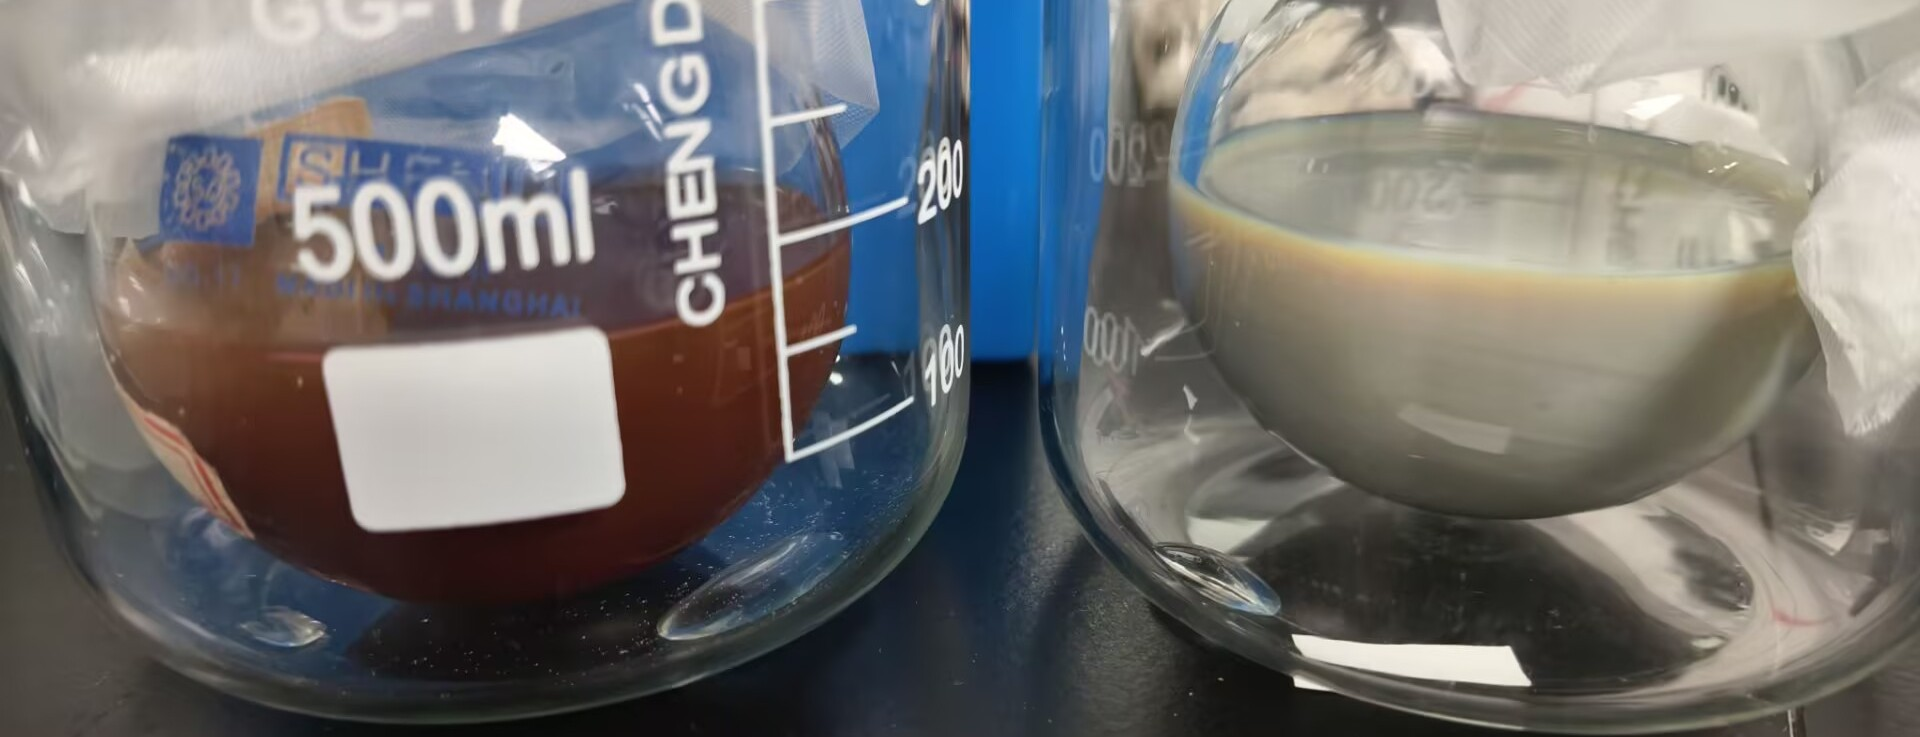
\includegraphics[width=0.7\linewidth]{src/img/sample_photo.jpg}
  \caption{{\zihaoWu 金、银纳米粒子样品的外观（左：AuNP，右：AgNP）}}
  \label{fig:sample}
\end{figure}

SEM 结果如图~\ref{fig:sem} 所示。为便于与参考报告中的形貌分析保持一致，图中选取同一编号的 AgNP 与 AuNP 样品进行对比。AuNP 样品整体分散性较好，颗粒以近球形或短椭球形为主，代表性尺寸约 50--70 nm，粒子边界较清楚。相比之下，AgNP 样品更易形成团簇，图中常见由近球形小颗粒堆积形成的花球状或葡萄串状聚集体，代表性表观尺寸多在几十纳米量级。该差异说明在相近制备条件下，银纳米粒子表面稳定性和成核/长大过程更容易受到局部浓度、离子强度和干燥过程影响；团聚也会导致等离激元耦合增强，使吸收峰展宽或红移。结合溶液颜色观察，AuNP 的红色调与金纳米粒子可见光区 LSPR 吸收相符，AgNP 的灰绿/灰蓝色则提示其分散性和粒径分布较 AuNP 更复杂。

\begin{figure}[h]
  \centering
  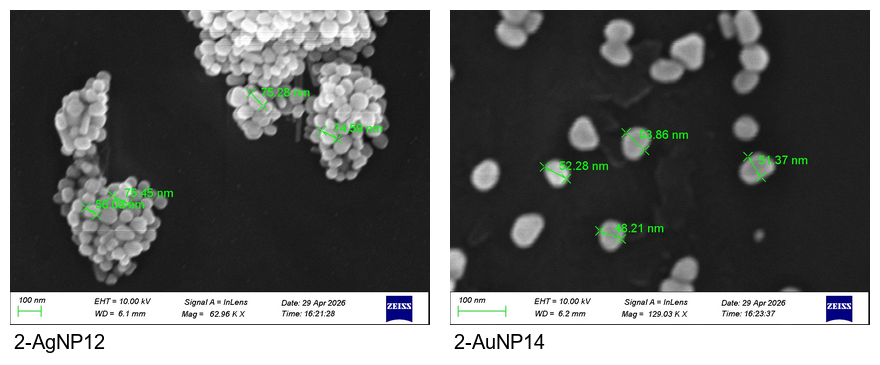
\includegraphics[width=0.82\linewidth]{src/img/sem_overview.png}
  \caption{{\zihaoWu 金、银纳米粒子样品的 SEM 形貌对比}}
  \label{fig:sem}
\end{figure}

\subsection{金、银纳米粒子的紫外--可见吸收特征}

图~\ref{fig:uvvis} 汇总了 3 条有效 AuNP 和 4 条 AgNP 的实测吸收曲线；其中一条 AuNP 数据因保存异常而与另一条曲线完全重复，未纳入绘图和讨论。有效 AuNP 曲线的最大吸收峰位于约 523--532 nm，其中 G6-1 Au 600 曲线在 532 nm 处出现最明显的 LSPR 峰，峰形较集中且长波侧拖尾较弱，说明该样品中金纳米粒子的粒径分布相对较窄、团聚程度较低；另外两条 Au 曲线峰位在 523--524 nm，可能对应粒径略小或局部介质环境不同的胶体。AgNP 的主峰主要位于约 415--434 nm，且部分曲线在主峰附近表现出更宽的峰形。由此可见，AuNP 的 LSPR 位于更长波长区域，而 AgNP 的主吸收处于蓝紫光附近；AgNP 峰形更宽、峰位波动更明显，与 SEM 中观察到的团聚和粒径分布较宽相互印证。

\begin{figure}[h]
  \centering
  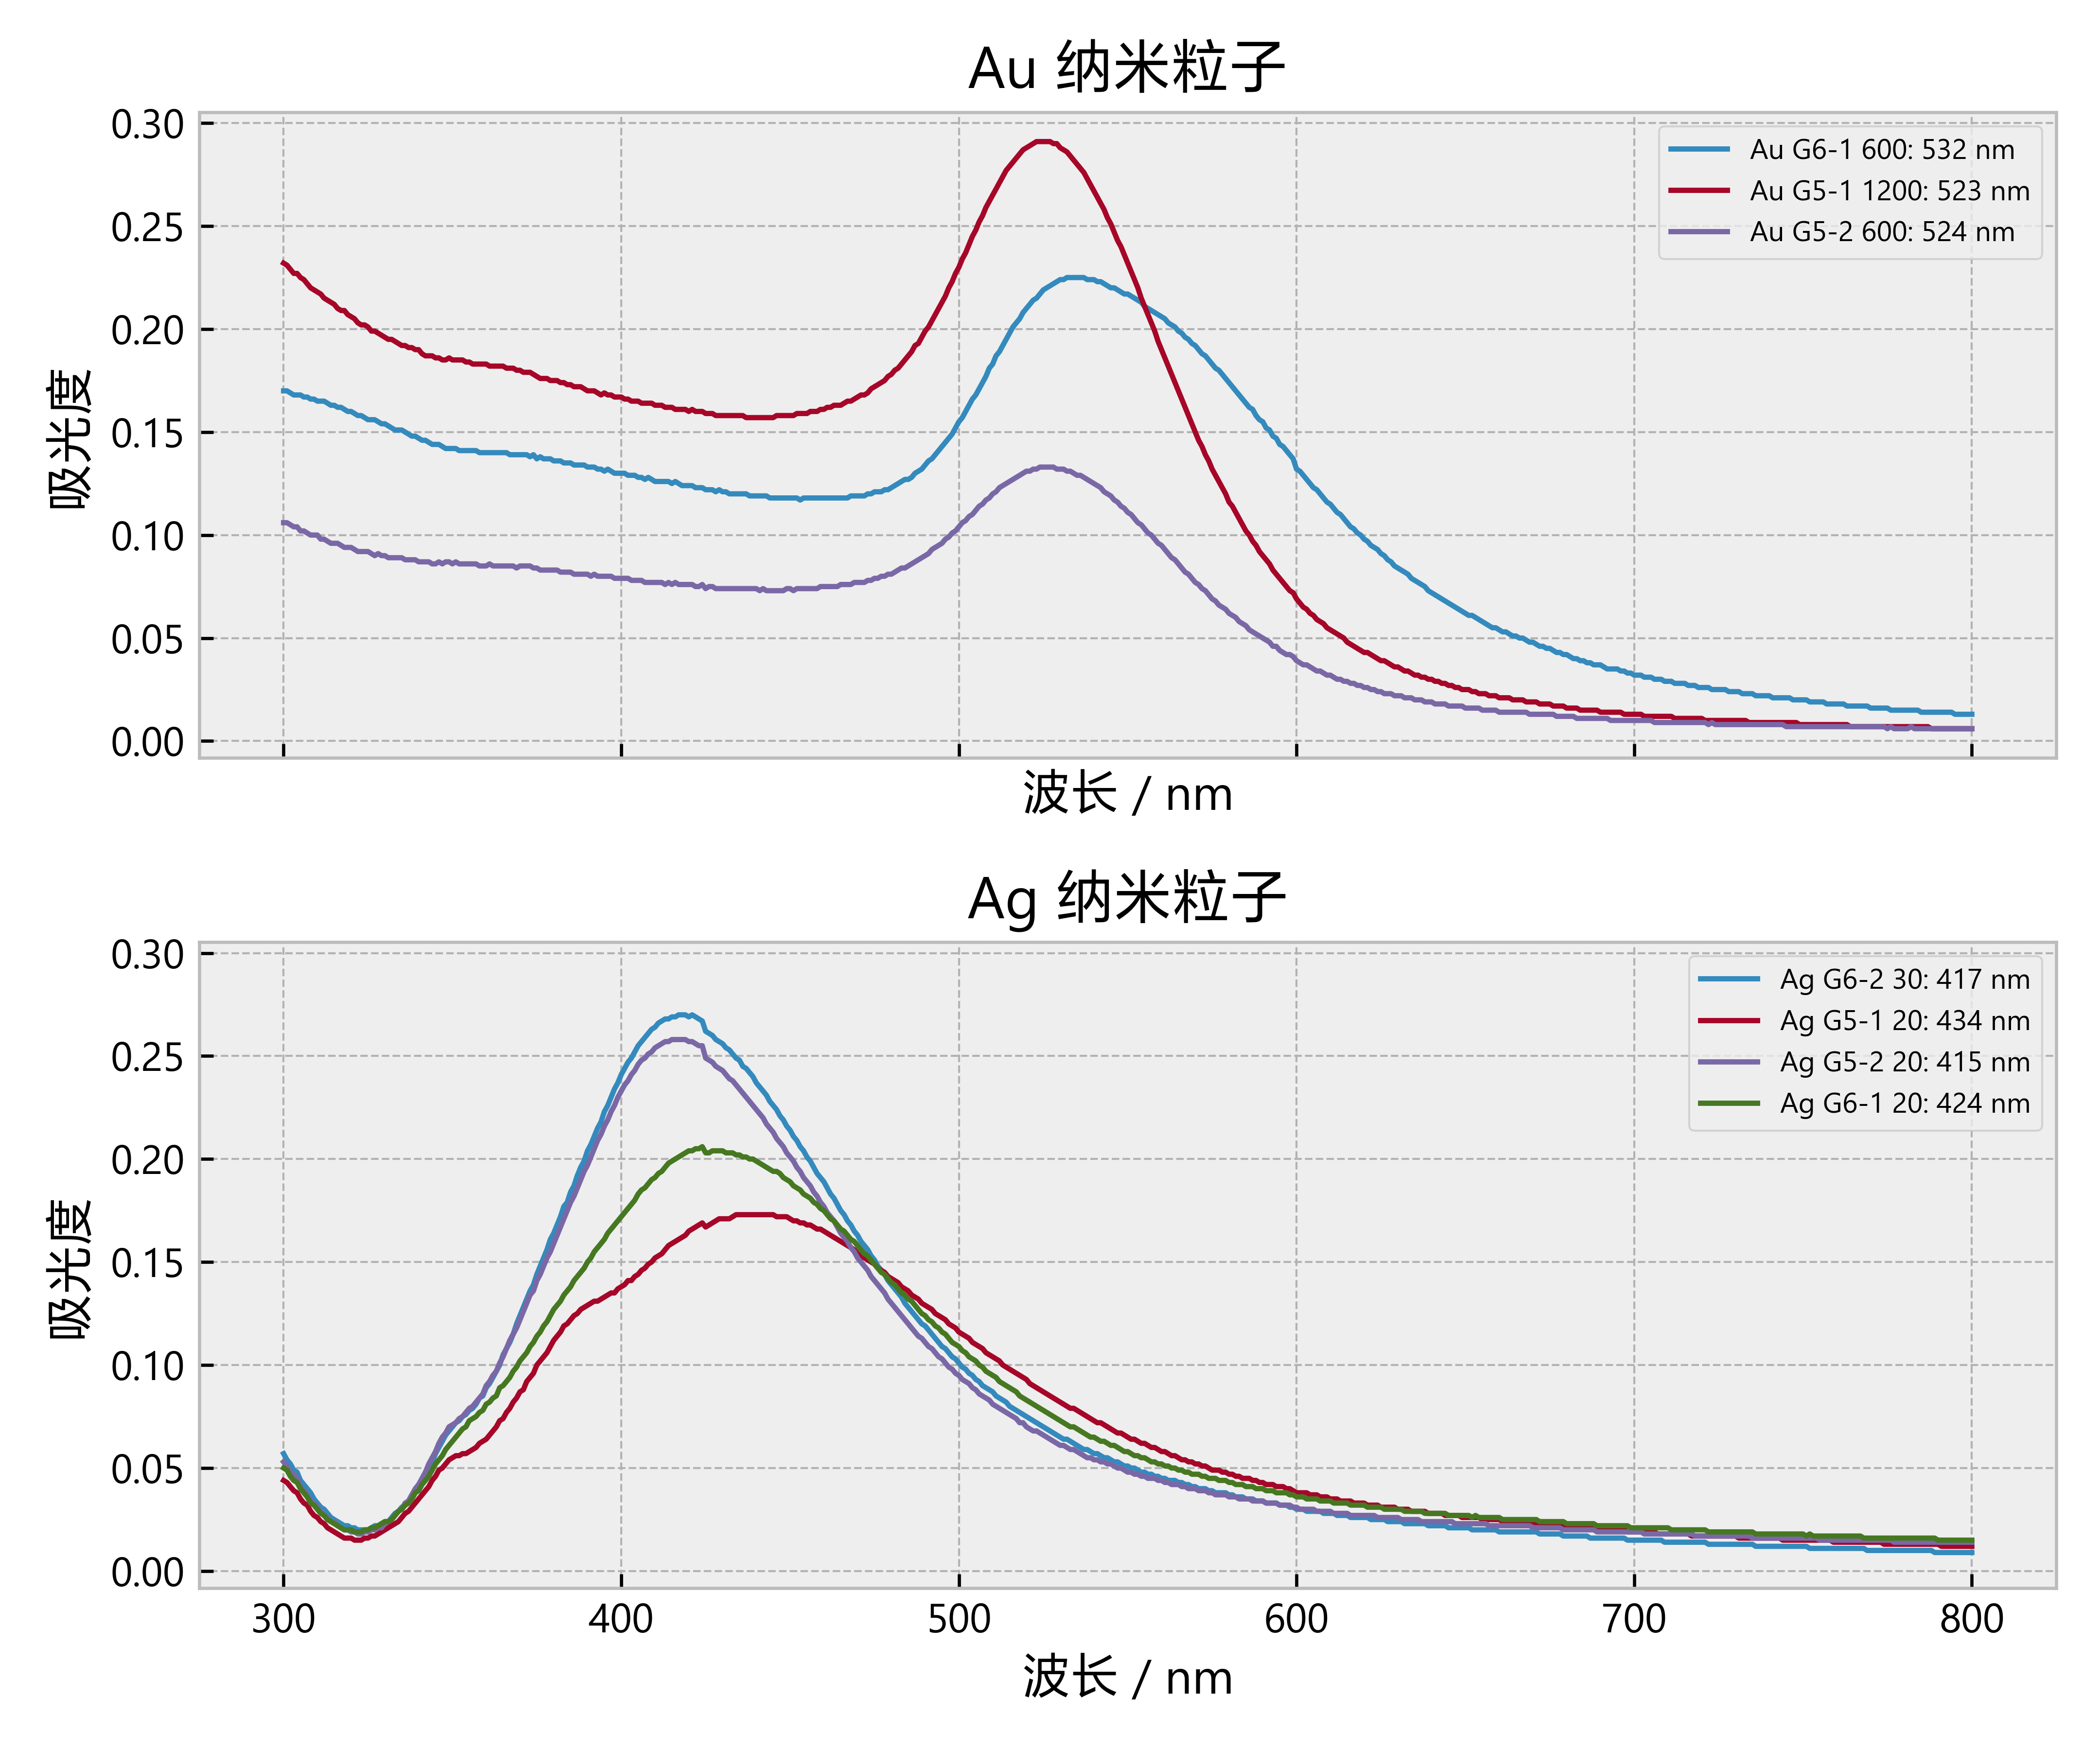
\includegraphics[width=0.9\linewidth]{src/img/uvvis_au_ag_reference.png}
  \caption{{\zihaoWu 金、银纳米粒子的实测紫外--可见吸收曲线}}
  \label{fig:uvvis}
\end{figure}

\subsection{拉曼光谱用于宝石样品鉴别}

真/仿钻石和真/仿翡翠的拉曼谱如图~\ref{fig:gem} 所示。真钻石在约 1335 cm$^{-1}$ 处出现单一尖锐强峰，对应金刚石晶格的一阶拉曼特征；仿钻样品则在约 778 cm$^{-1}$ 和 966 cm$^{-1}$ 附近出现两个主要峰，未出现钻石的 1332 cm$^{-1}$ 特征峰，因此可直接判定其晶体组成与真钻不同。翡翠样品中，真翡翠可见约 365、685 和 1024 cm$^{-1}$ 等多处矿物特征峰，而仿翡翠主要表现为较强背景和弱特征峰，说明其结构或组成与天然翡翠存在显著差别。该结果表明，拉曼光谱具有样品制备简单、峰位指纹性强的优点，适合用于宝石类样品的快速无损鉴别。

\begin{figure}[h]
  \centering
  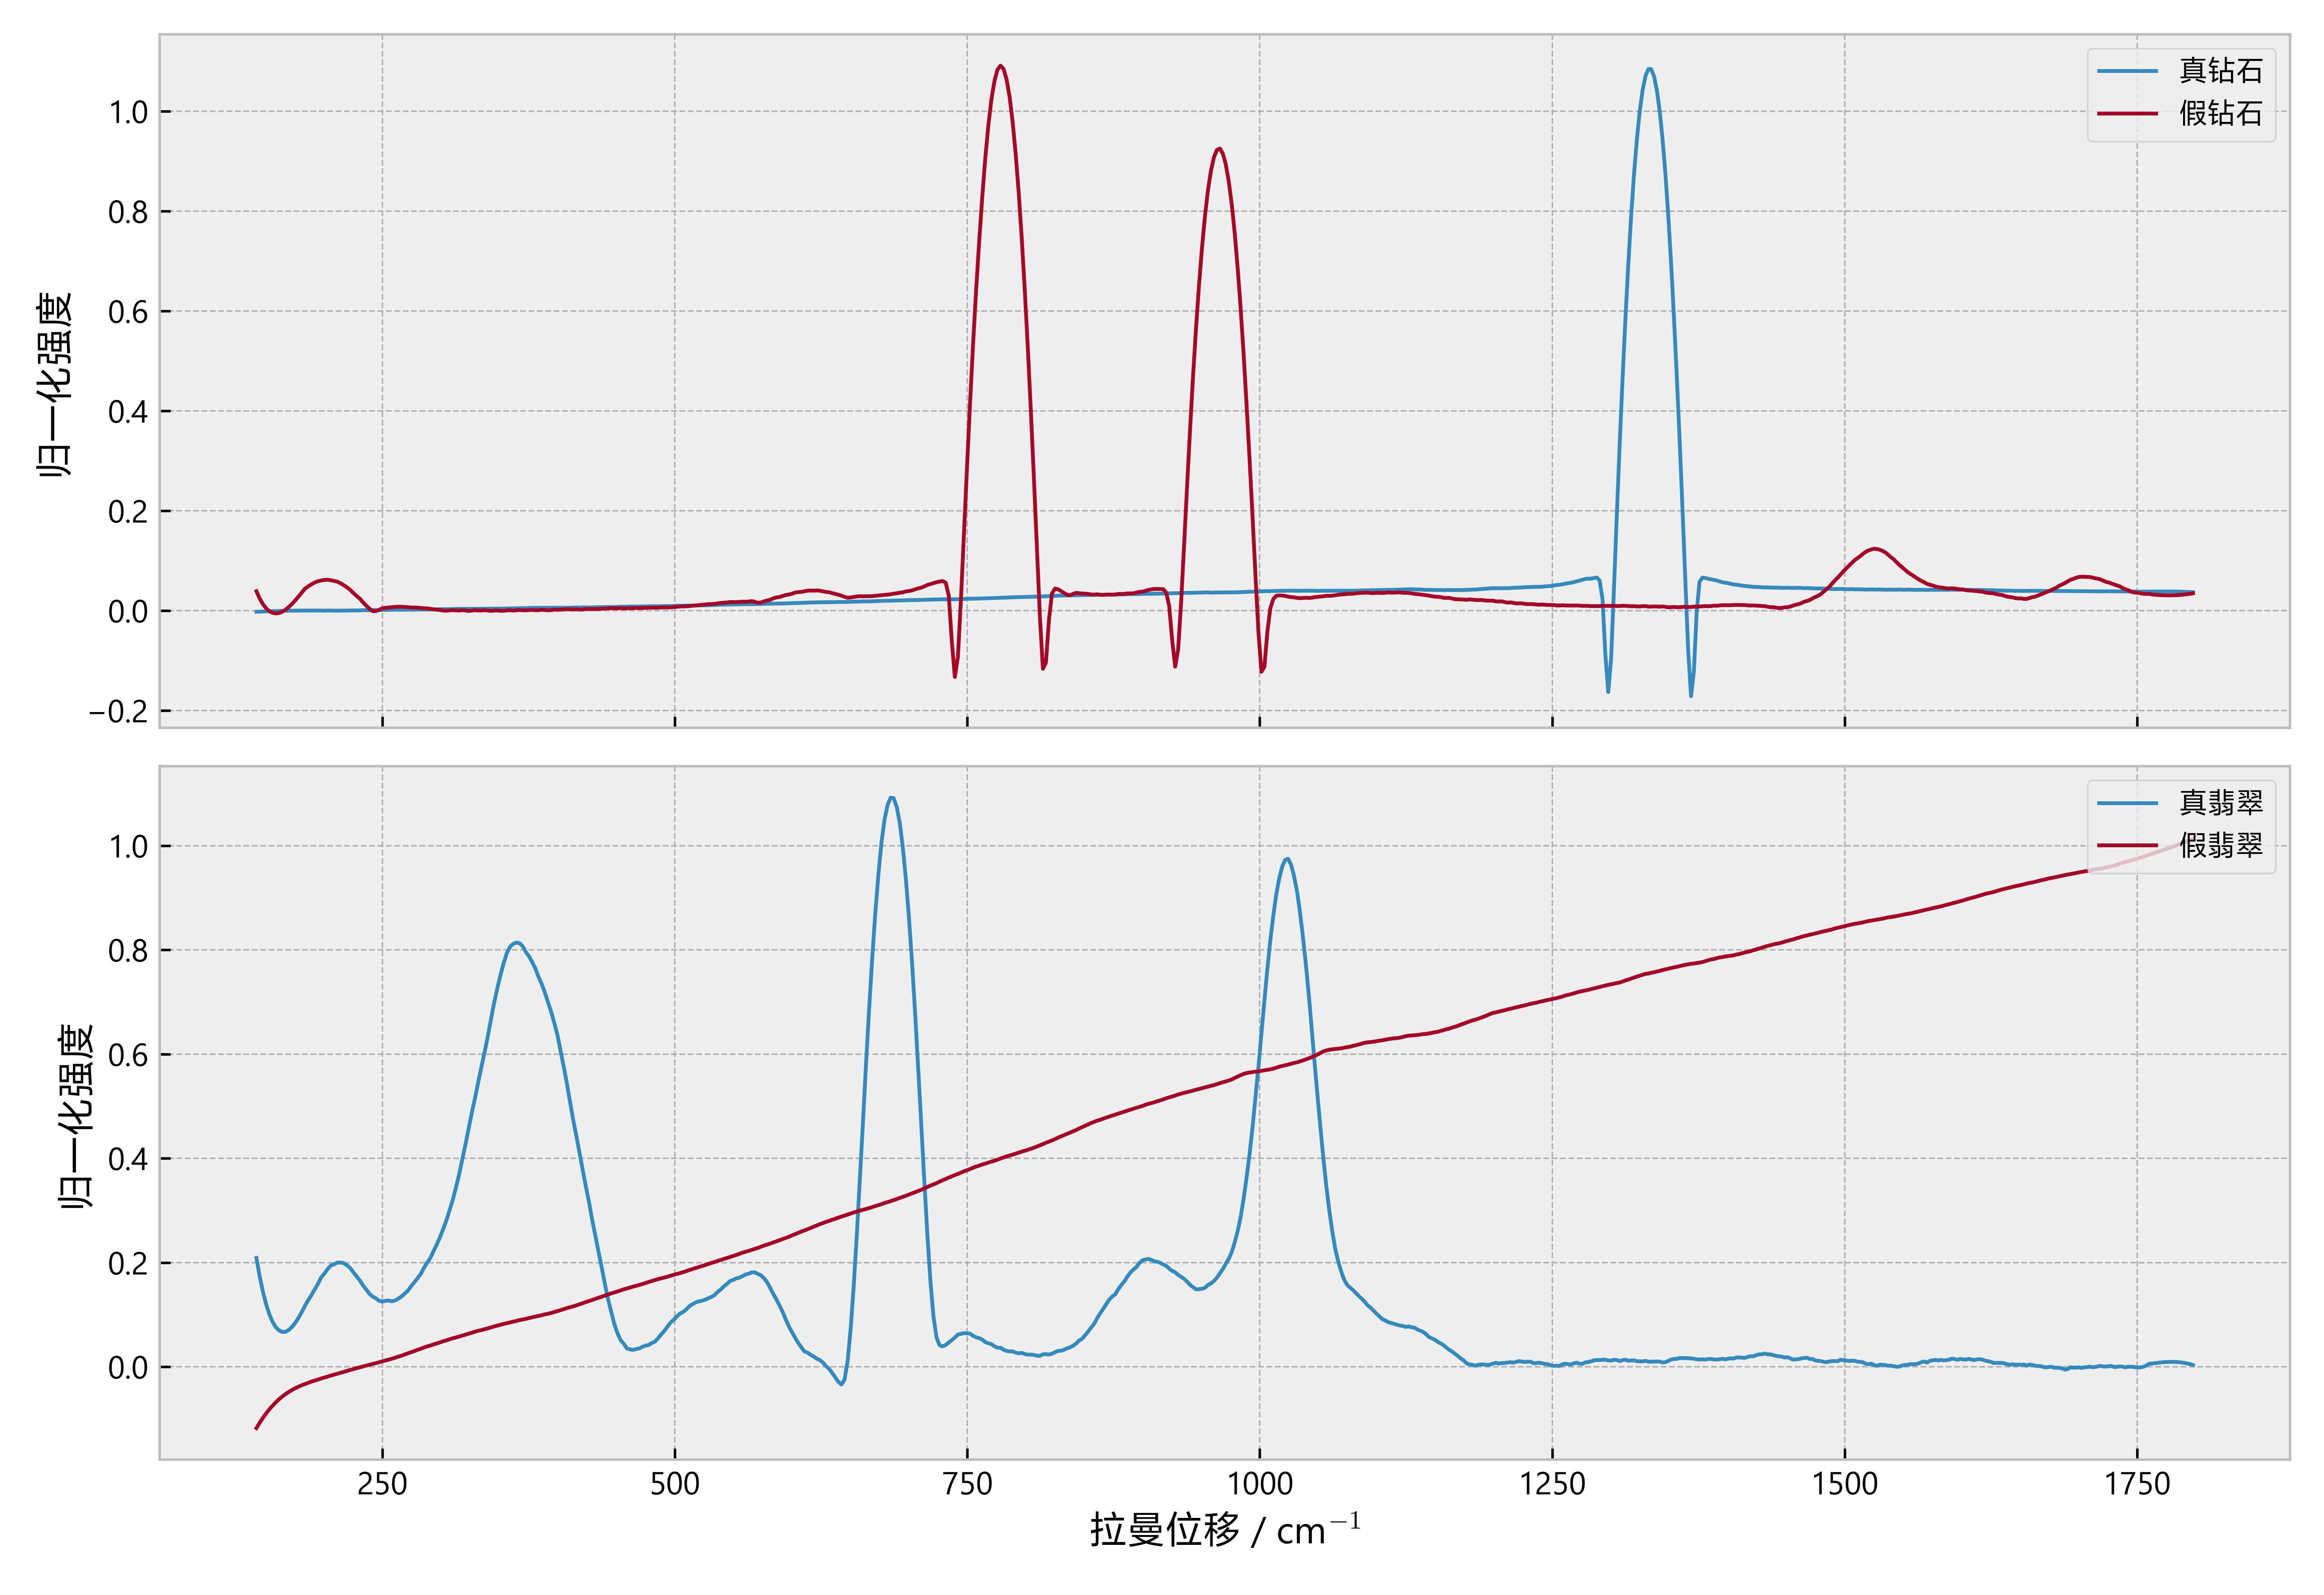
\includegraphics[width=0.82\linewidth]{src/img/raman_gem_comparison.png}
  \caption{{\zihaoWu 真/仿钻石与真/仿翡翠的拉曼光谱}}
  \label{fig:gem}
\end{figure}

\subsection{孔雀石绿的 SERS 检测}

孔雀石绿在不同增强条件下的谱图如图~\ref{fig:mg} 所示。未加入纳米粒子时，低浓度样品的拉曼峰较弱；加入 AgNP 后，1175、1378、1482 和 1610 cm$^{-1}$ 附近的特征峰明显增强；进一步加入 NaI 后，峰形在 0.1--10 mg/L 范围内更加清晰且重复出现。NaI 的作用可理解为改变 AgNP 表面电荷与吸附环境，诱导适度聚集并形成纳米间隙“热点”，从而增强局域电磁场。由于三种处理条件下主要峰位基本一致，说明增强过程并未改变孔雀石绿分子的基本振动结构，而主要提高了拉曼散射截面。

在 100 mg/L 条件下，部分谱图出现较强低波数背景和峰形异常，提示高浓度时可能发生吸附位点饱和、荧光背景增强或颗粒聚集状态改变。实际痕量检测更关注低浓度区域的可识别性，本实验中 AgNP 与 NaI 共同存在时，0.1 mg/L 样品仍能观察到孔雀石绿的多个特征峰，体现了 SERS 对染料分子的高灵敏检测能力。

\begin{figure}[htbp]
  \centering
  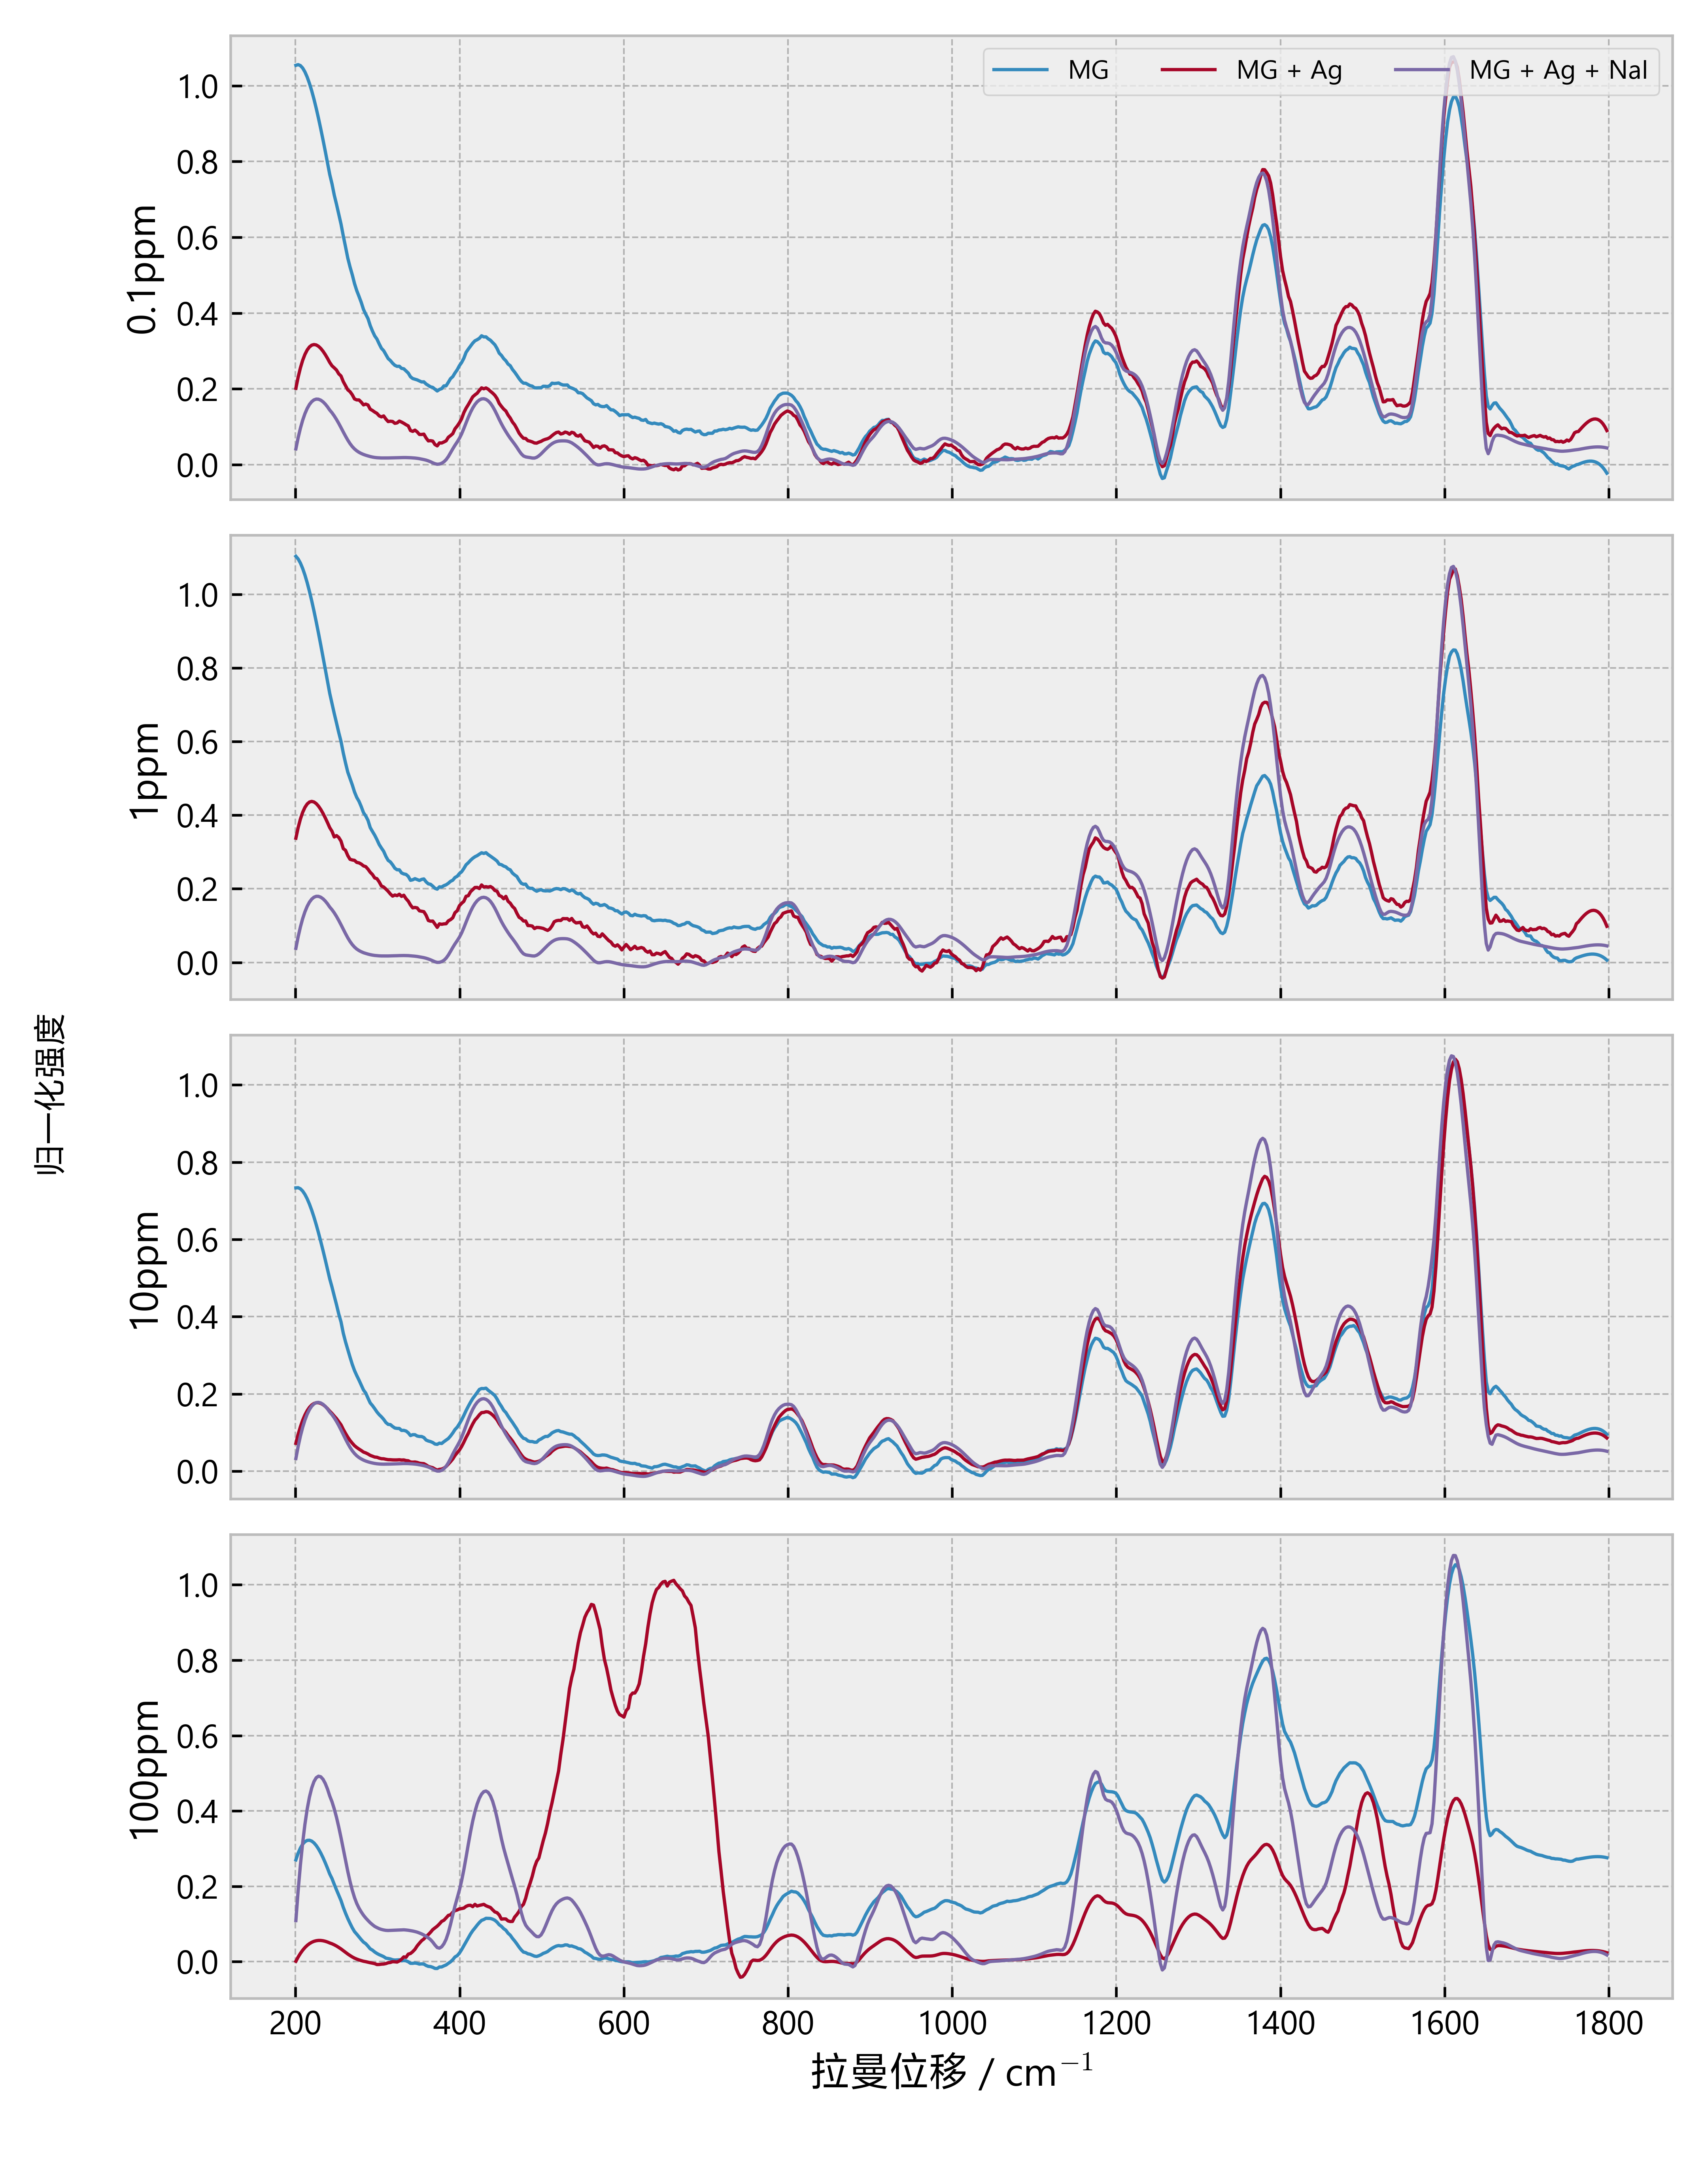
\includegraphics[width=0.9\linewidth]{src/img/sers_malachite_green.png}
  \caption{{\zihaoWu 孔雀石绿在不同浓度和增强条件下的拉曼/SERS 光谱}}
  \label{fig:mg}
\end{figure}

\newpage

\subsection{电位调控下的原位 SERS 响应}

电位序列 SERS 谱如图~\ref{fig:ec} 所示。测试先由 0 V 逐步调至 -0.70 V，随后回扫至 0 V。全序列中约 1614--1622 cm$^{-1}$ 和 1362--1379 cm$^{-1}$ 附近的主要峰持续存在，说明吸附分子的主体振动模式保持稳定；峰强随电位变化而改变，低波数区约 579--588 cm$^{-1}$ 的峰在较负电位下更容易分辨。回扫过程中相同标称电位下的峰强并不完全重合，提示界面吸附状态或纳米粒子聚集/电荷分布存在一定滞后。电位调控可能改变分子在金属表面的吸附取向、电子密度以及界面电荷转移贡献，因此主要表现为峰强变化而非大幅峰位漂移。该结果说明 SERS 不仅可用于痕量检测，也可用于跟踪电极/纳米粒子界面上的吸附和氧化还原过程。

\begin{figure}[h]
  \centering
  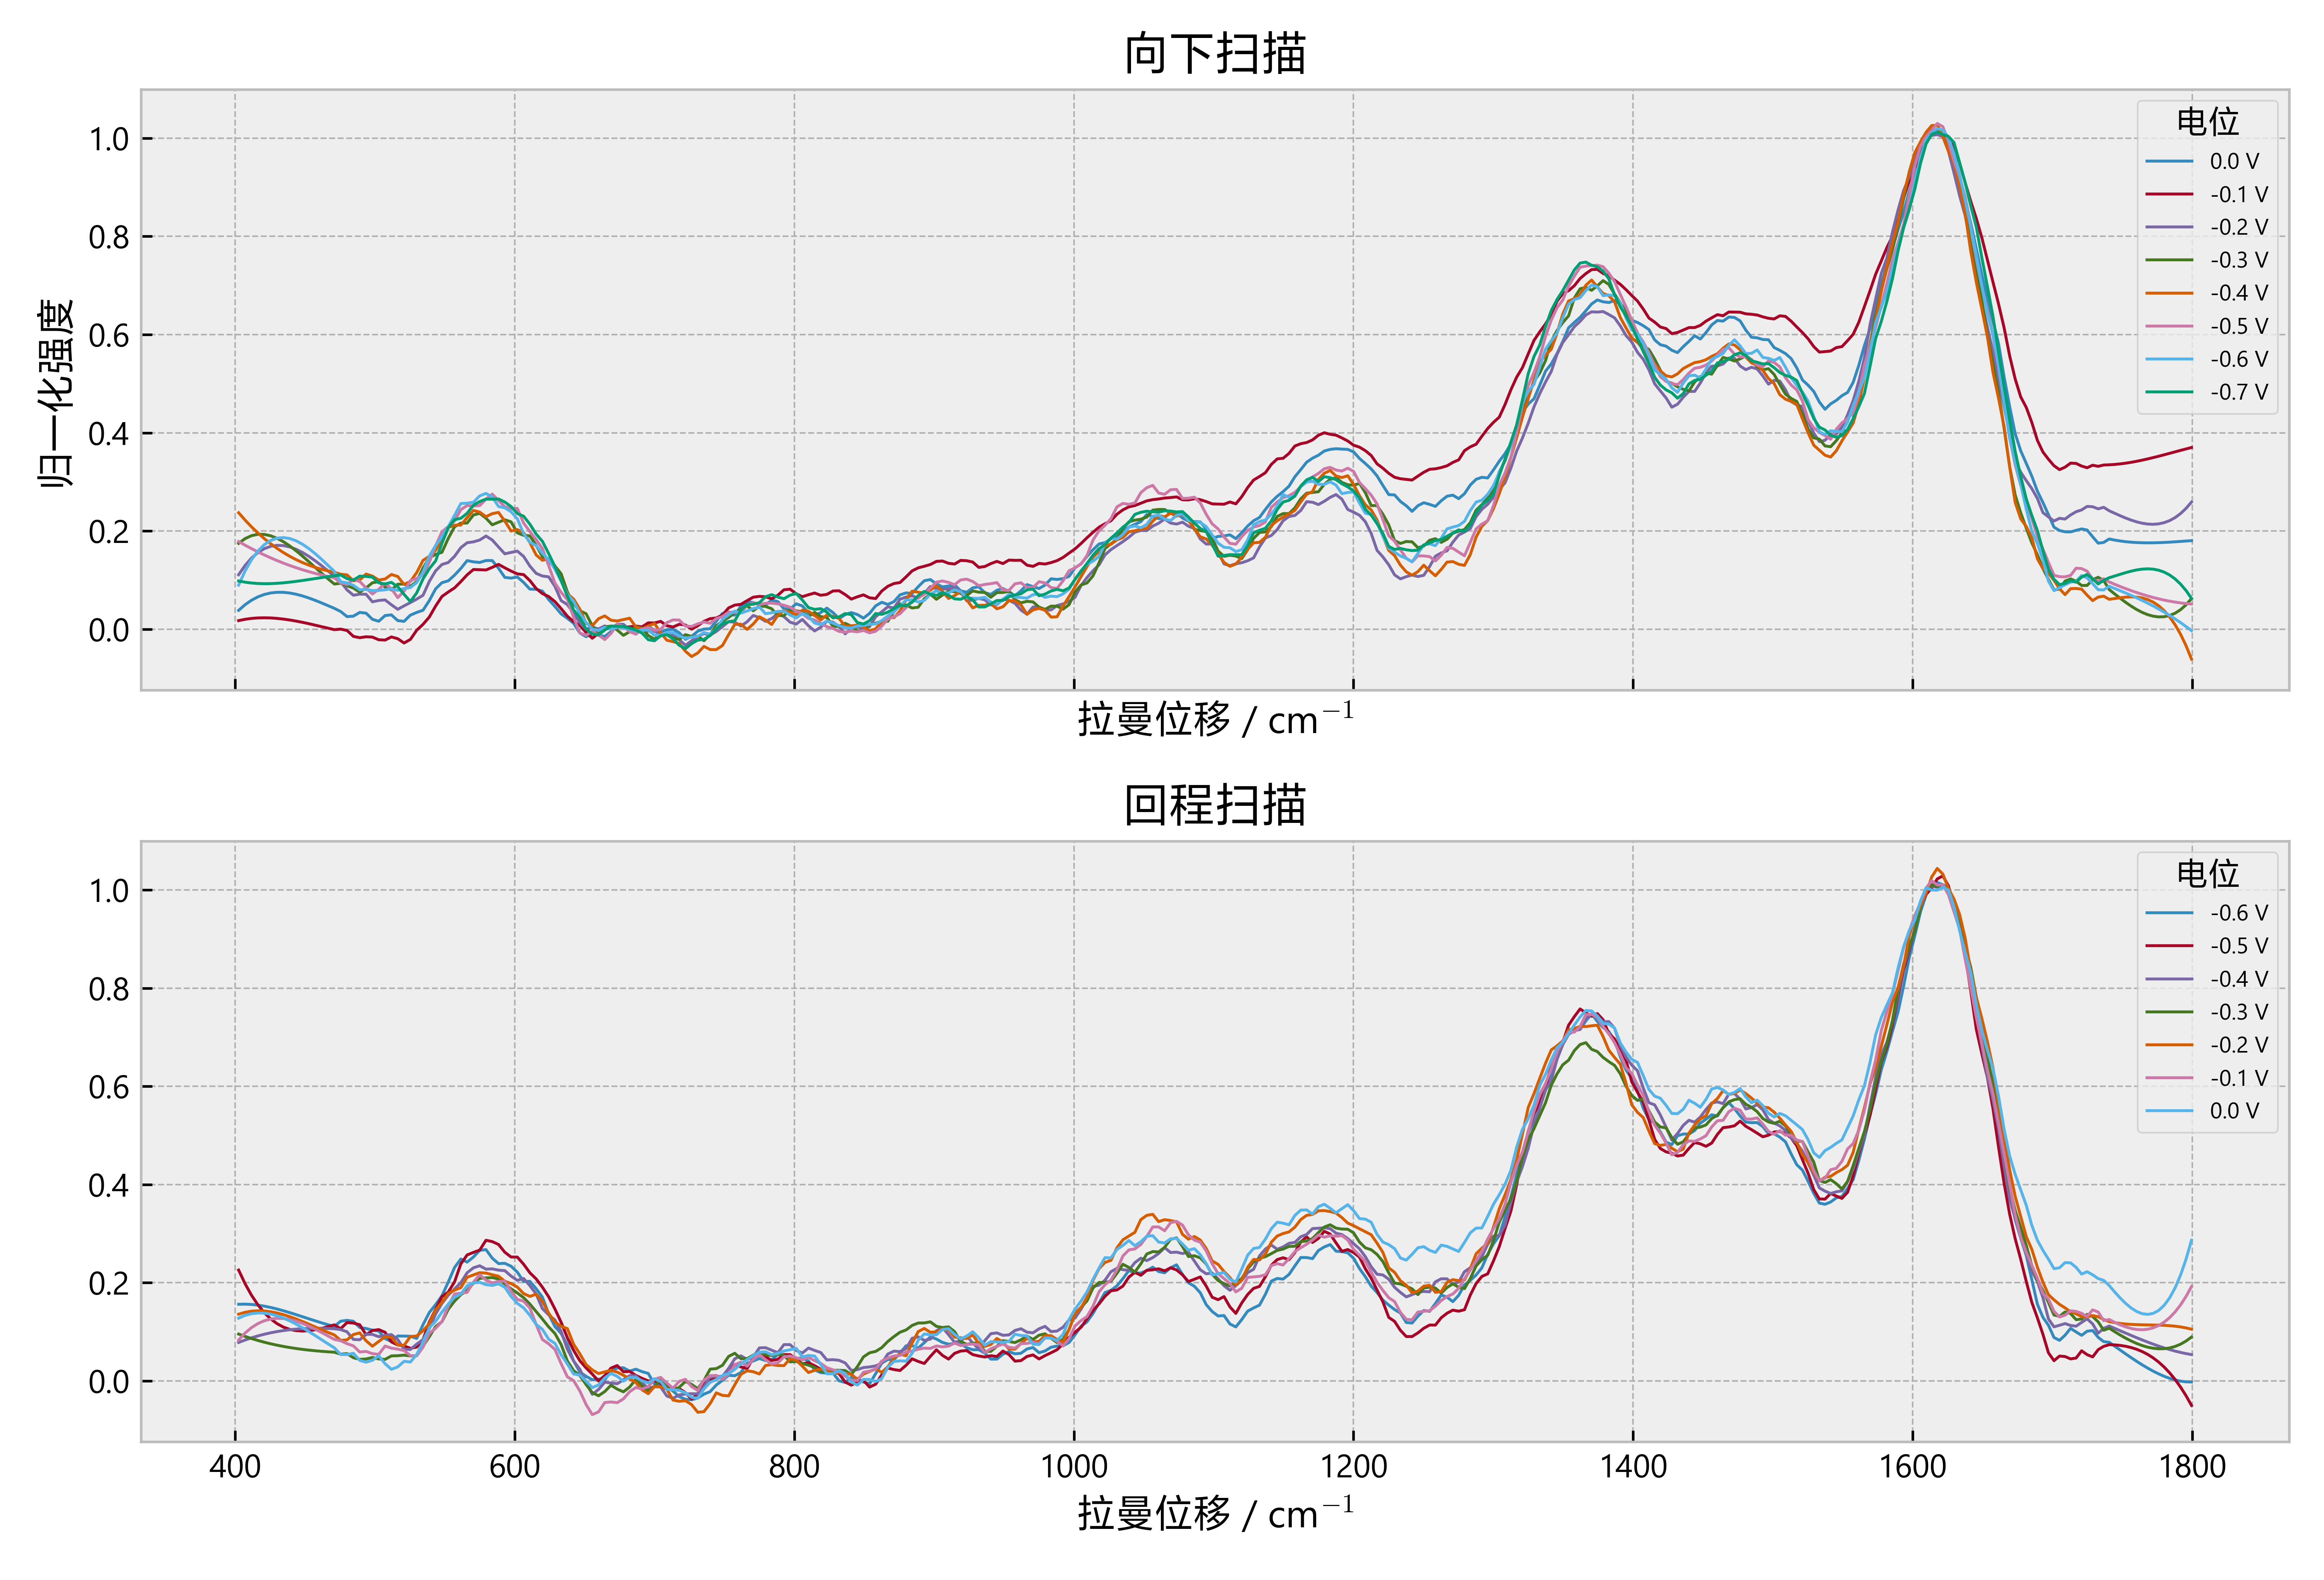
\includegraphics[width=\linewidth]{src/img/ec_sers_potential_series.png}
  \caption{{\zihaoWu 电位下扫及回扫过程中的原位 SERS 光谱}}
  \label{fig:ec}
\end{figure}

为进一步比较电位响应，选取约 588 cm$^{-1}$ 与 1618 cm$^{-1}$ 两个代表性峰计算归一化峰高，结果见图~\ref{fig:ecpeak}。两条峰强曲线在下扫和回扫过程中均出现起伏，且在转折点前后并非完全镜像，说明电化学调控下的 SERS 响应不仅取决于瞬时电位，还与吸附层重排、局部热点结构和电极界面历史有关。与堆叠谱图相比，峰强--电位曲线更直观地反映了电位对界面增强效应的调制。

\begin{figure}[h]
  \centering
  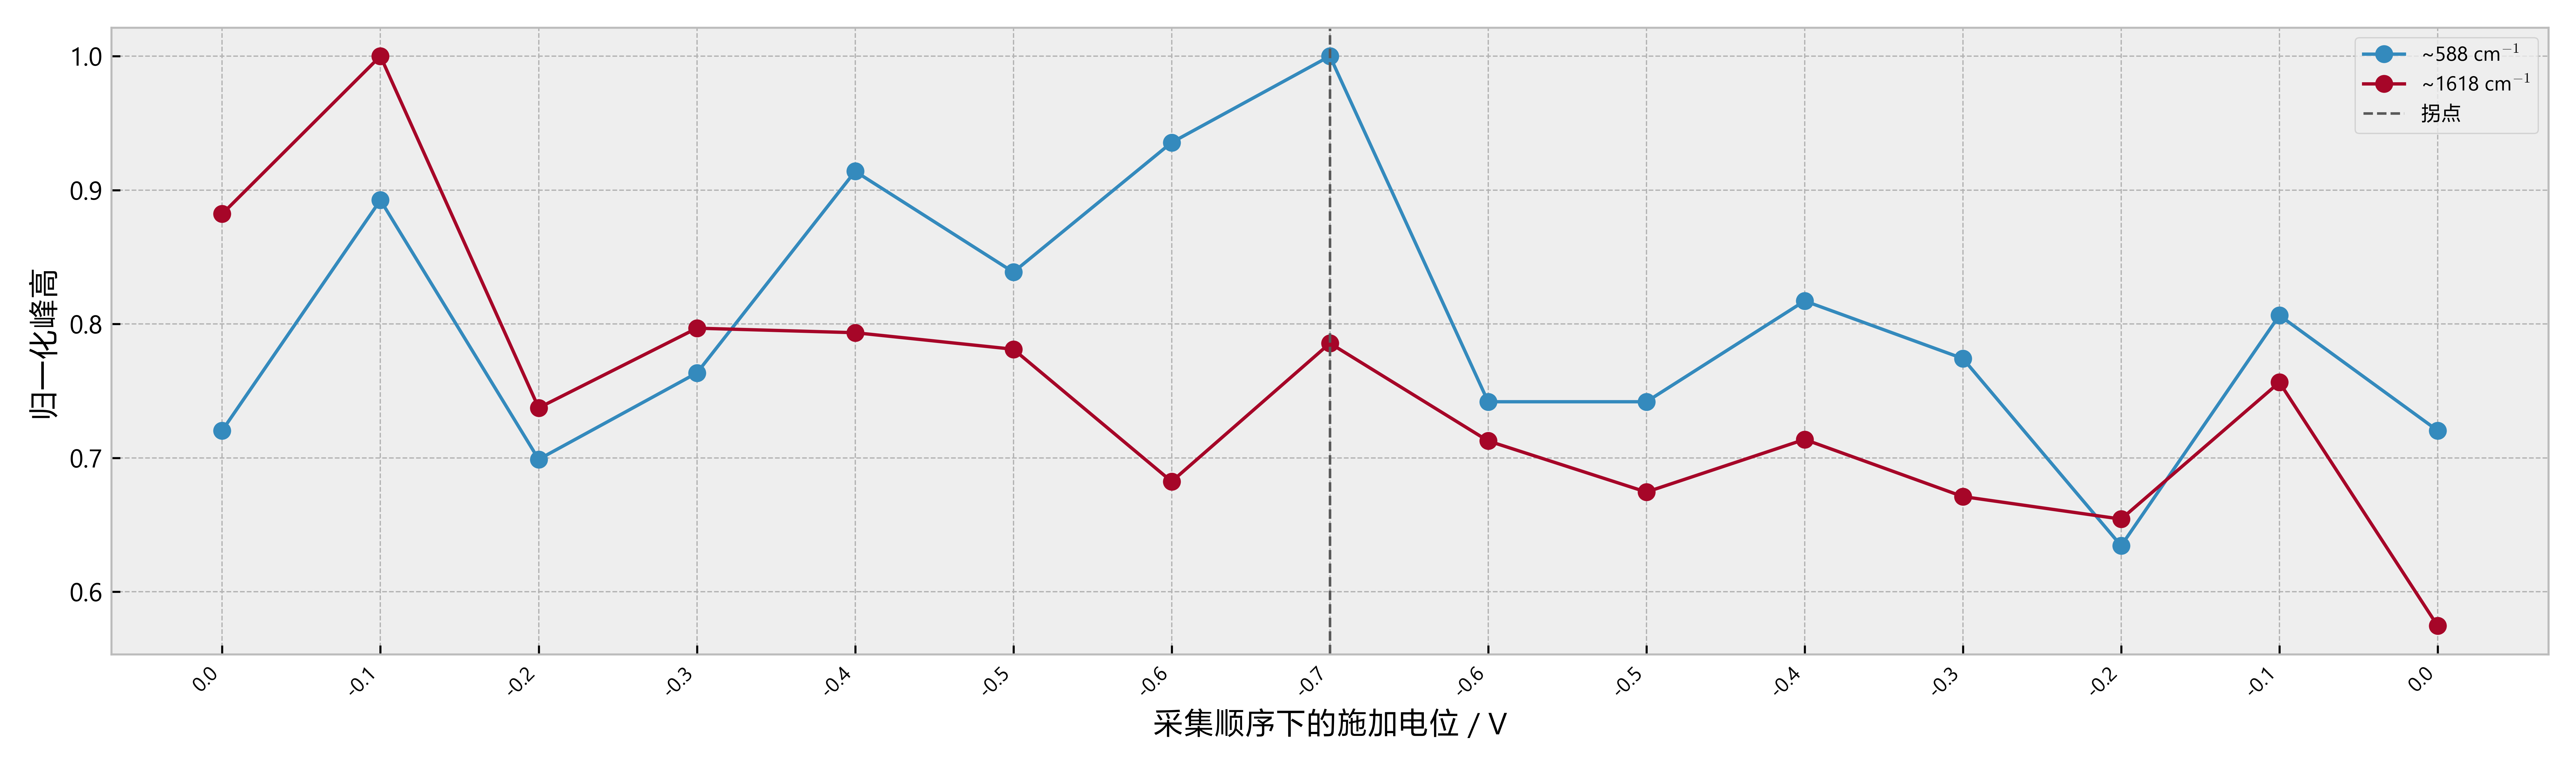
\includegraphics[width=\linewidth]{src/img/ec_sers_peak_trend.png}
  \caption{{\zihaoWu 原位 SERS 代表性峰强随电位扫描顺序的变化}}
  \label{fig:ecpeak}
\end{figure}

\newpage

\section{思考题}
\vspace{-0.5em}

\begin{enumerate}[label=\textbf{\arabic*.},leftmargin=2.5em]
  \item \textbf{为何金属纳米粒子的颜色与它们在宏观尺度上的颜色有所不同？}

        宏观金属的颜色主要来自能带结构对不同波长光的反射和吸收，而贵金属纳米粒子的颜色由 LSPR 主导。纳米粒子尺寸小于或接近可见光波长时，表面自由电子可被入射光驱动产生集体振荡，并在特定波长产生强吸收和散射。该共振波长对粒径、形貌、介质折射率和颗粒间距都很敏感，因此金纳米粒子常呈红色，银纳米粒子可呈黄色、灰绿或蓝灰色；当颗粒增大或团聚时，共振耦合增强，颜色也会发生变化。

  \item \textbf{描述金纳米粒子和银纳米粒子一步法合成的化学反应原理。为什么这种方法能够有效合成纳米粒子？}

        一步法的核心是将金属盐中的 Au(III) 或 Ag(I) 还原为零价金属原子，随后金属原子成核并长大为纳米粒子。柠檬酸钠在体系中同时承担还原剂和稳定剂作用：一方面提供电子使金属离子还原，另一方面以羧酸根吸附在颗粒表面，使颗粒带电并产生排斥作用。加热可提高还原速率，使单体浓度迅速超过成核阈值，形成较集中的晶核；随后单体主要沉积在已有晶核上，从而在较短时间内得到胶体纳米粒子。

  \item \textbf{探讨反应物浓度、pH 值、反应温度等参数对纳米粒子大小和形状的影响。}

        金属盐浓度升高会提高单体生成速率，若还原剂不足或稳定剂覆盖不充分，易造成粒径增大和团聚；若成核数量显著增加，则平均粒径可能减小。pH 会影响柠檬酸根的解离状态、还原能力和颗粒表面电荷，进而改变成核速率和胶体稳定性。温度升高通常加快还原和扩散过程，有利于快速成核，但过高温度或局部过热也可能导致生长不均、奥斯特瓦尔德熟化或聚集。对于各向异性颗粒，配体选择性吸附还会改变不同晶面的生长速率，从而影响棒状、片状或多面体形貌。

  \item \textbf{解释种子法合成金纳米粒子的原理。与一步法相比，金种法有什么优势和缺点？}

        种子法先制备小尺寸、数量较多且相对均一的金晶种，再在含金属前驱体、温和还原剂和配体的生长液中进行外延生长。由于成核阶段与长大阶段被分开，后续反应更倾向于在已有晶种表面沉积，而不是重新均相成核，因此更容易控制粒径、形貌和单分散性。其优势是可获得尺寸可调、形貌复杂的纳米结构；缺点是步骤较多，对晶种质量、加入顺序、配体浓度和温度更敏感，重复性和操作成本不如一步法简单。

  \item \textbf{如何通过紫外--可见吸收光谱来确定合成纳米粒子的尺寸？解释吸收峰位置和纳米粒子尺寸之间的关系。}

        紫外--可见吸收光谱中贵金属纳米粒子的 LSPR 峰可用于判断粒径和分散状态。对于近球形 AuNP，粒径较小时吸收峰通常位于 520 nm 左右；粒径增大、形貌拉长或团聚增强时，峰位向长波方向移动并展宽。AgNP 的主吸收峰常位于 400 nm 左右，粒径分布变宽或颗粒间耦合会导致峰形展宽、肩峰或红移。严格粒径需要结合标准曲线、Mie 理论拟合或 SEM/TEM 统计，但峰位和半峰宽可快速反映样品是否均一、是否发生明显聚集。

  \item \textbf{SEM 如何帮助确认纳米粒子的形状、大小和分布？制样时应注意哪些关键点？}

        SEM 可直接给出颗粒在基底上的形貌图像，观察其是否为球形、棒状、片状或团聚体，并可通过标尺和软件测量获得代表性尺寸。多视野统计还能估计粒径分布和团聚程度。制样时应保证样品足够稀释并充分分散，避免滴加过浓导致干燥后咖啡环和团聚；基底应洁净、导电并固定牢靠；样品必须充分干燥，避免残留溶剂污染真空系统；对绝缘或易荷电样品可考虑喷镀导电层或降低加速电压，以减少充电和束流损伤。
\end{enumerate}

\section{结论}
\vspace{-0.5em}

本实验通过液相还原法制备了金、银纳米粒子，并利用 SEM、UV-Vis、拉曼和 SERS 方法考察了其结构与分析应用。SEM 显示 AuNP 较分散、粒形较规则，而 AgNP 更易形成团聚体；UV-Vis 峰位整理显示有效 AuNP 曲线的 LSPR 主要集中在约 523--532 nm，AgNP 主峰集中在约 415--434 nm，二者与颜色和形貌差异相互印证。常规拉曼光谱可清晰区分真/仿钻石和真/仿翡翠，说明分子或晶格振动峰具有良好的指纹识别能力。孔雀石绿检测中，AgNP 与 NaI 的协同作用显著增强了特征峰，使低浓度样品仍具备可识别谱形。电位调控 SERS 进一步表明，界面电荷状态会影响吸附分子的峰强响应，并在回扫中表现出一定历史效应。总体而言，贵金属纳米粒子的尺寸、分散性和聚集状态共同决定其光学与 SERS 性能，合成控制与表征结果需要结合分析，才能服务于可靠的纳米传感应用。

\vspace{2em}
{\footnotesize
  \setstretch{1}
  \begin{thebibliography}{9}
    \bibitem{Willets2007}
    K. A. Willets and R. P. Van Duyne.
    \textit{Annu. Rev. Phys. Chem.}, \textbf{2007}, 58: 267--297.

    \bibitem{Mayer2011}
    K. M. Mayer and J. H. Hafner.
    \textit{Chem. Rev.}, \textbf{2011}, 111(6): 3828--3857.

    \bibitem{Pratap2025}
    A. Pratap \textit{et al.}
    \textit{ACS Omega}, \textbf{2025}. DOI: 10.1021/acsomega.4c11045.

    \bibitem{CoreShell2025}
    \textit{Journal of Manufacturing and Materials Processing}, \textbf{2025}, 9: 131.

    \bibitem{Zhou2023}
    X. Zhou, S. Chen, Y. Pan, Y. Wang, N. Xu, Y. Xue, X. Wei and Y. Lu.
    \textit{Biosensors}, \textbf{2023}, 13: 766.

    \bibitem{Deniz2019}
    F. Deniz.
    \textit{Materials Letters}, \textbf{2019}, 256: 126940.
  \end{thebibliography}
}

\vspace*{\fill}
\noindent{\zihaoWu 评语（Remarks）：}
\vspace{2em}
\begin{center}
  {\zihaoWu\bfseries 指导教师（Instructor）\hspace{8em} 日期（Date）}
\end{center}
\vspace{1.5cm}

\end{document}
